% This must be in the first 5 lines to tell arXiv to use pdfLaTeX, which is strongly recommended.
\pdfoutput=1
% In particular, the hyperref package requires pdfLaTeX in order to break URLs across lines.

\documentclass[11pt]{article}

% Remove the "review" option to generate the final version.
\usepackage{acl}

% Standard package includes
\usepackage{times}
\usepackage{latexsym}

% For proper rendering and hyphenation of words containing Latin characters (including in bib files)
\usepackage[T1]{fontenc}
% For Vietnamese characters
% \usepackage[T5]{fontenc}
% See https://www.latex-project.org/help/documentation/encguide.pdf for other character sets

% This assumes your files are encoded as UTF8
\usepackage[utf8]{inputenc}

% This is not strictly necessary, and may be commented out,
% but it will improve the layout of the manuscript,
% and will typically save some space.
\usepackage{microtype}

\usepackage{amsmath}
\usepackage{graphicx}
\usepackage{hhline}
\usepackage{multirow}
\usepackage[capitalize,nameinlink]{cleveref}
\hypersetup{colorlinks = true, citecolor = blue, linkcolor = blue}
\definecolor{blue}{HTML}{00a4ff}
\usepackage{subcaption}
\usepackage{placeins}

% If the title and author information does not fit in the area allocated, uncomment the following
%
%\setlength\titlebox{<dim>}
%
% and set <dim> to something 5cm or larger.

\renewcommand{\emph}[1]{\textcolor{blue}{#1}}

\title{Homework 2}
\author{Pedro Matias \\
\textsf{pmatias@uci.edu}}

\begin{document}

\noindent{\Large \textbf{Homework 2}}

\noindent\textbf{Pedro Matias}

\noindent\textsf{pmatias@uci.edu}

% \maketitle
% \noindent
% \begin{minipage}[t]{.5\textwidth}
% {\Large \textbf{Homework 2}\\[1em]Homework 1}
% \end{minipage}% This must go next to `\end{minipage}`
% \begin{minipage}[t]{.5\textwidth}
% \begin{flushright}
%     Pedro Matias\\
%     23201116\\
%     {\small \texttt{pmatias@uci.edu}}
% \end{flushright}
% \end{minipage}

\setcounter{section}{2}

\section*{2.1$\;\;$ Implement an $n$-gram Language Model}

We implemented two distinct $n$-gram models: one does not use any sort of UNK substitution, and the other uses the classic UNK substitution for rare words (details below). To account for rare $n$-grams we used Laplace smoothing in both models with varying values of $\lambda$ (see next section). To account for OOV words in the \textbf{first} model, we leverage the usage of Laplace smoothing, by defining (for some $\lambda$) the distribution $p(w\mid \textsf{context})$ as follows
\[
\frac{C(\textsf{context}\cdot w) + \lambda}{C(\textsf{context}) + \lambda(V + \textsf{NOOV})}
\]
Notice the addition of \texttt{NOOV} in the denominator. The intuition behind this is the following. We resolve OOV words by ``pretending'' we have seen them $\lambda$ times, one for each occurrence in a fictitious $n$-gram, which is itself resolved by ``pretending'' we have seen it $\lambda$ times, using Laplace smoothing. But having pretended that we have seen all OOV words, we need to increase the size of our vocabulary accordingly and, thus, the addition of \texttt{NOOV} in the denominator. This model is much simpler than the second model and it managed to improve upon the unigram model for $n=2$, even though it didn't perform as good as the second model.

For the \textbf{second} model, we define non-UNK words according to the parameter $\textsf{voc\_ratio}$, which defines the fraction of the training vocabulary which occurs most frequently in the training corpus. We use Adjusted Perplexity in our hyper-parameter search, so as to minimize bias caused by high probability UNK tokens, by adjusting $p(\mathrm{UNK}\mid \mathrm{context})$ with a multiplicative factor of $1/\mathrm{NOOV}$, where $\mathrm{NOOV}$ is the number of words OOV. 


\paragraph{Implementation details: }

\begin{itemize}
  \item To simplify the implementation, we keep counts for all $n$-grams, as well as all $(n-1)$-grams. The latter are are used to count the number of occurrences of the given \textsf{context}. Notice that this is equivalent to counting all $n$-grams that start with \textsf{context}, since we append a \texttt{END\_OF\_SEQUENCE} token to each sequence.
  \item To avoid numerical underflow, we perform all computations (except for counting $n$-grams) in $\lg$ space.
  \item We add $n-1$ tokens \texttt{START\_OF\_SEQUENCE} in the beginning of each sequence (in both training and prediction), so we can simplify the handling of word probability distributions conditioned on fractional contexts (i.e. of size less than $n-1$).
\end{itemize}


\section*{2.2$\;\;$ Hyper-parameter Search}\label{sec:search}

For the first ``no-UNKs'' model we simply varied $n$ and $\lambda$ -- see \cref{fig:nounks} for ranges and a comparison against the unigram model. We did not conduct any finer hyper-parameter search since this model performed worse than the one using UNKs.

For the second model, we varied $n$, $\lambda$ and \textsf{voc\_ratio}. In anticipating that large $n$-grams would yield too much sparsity (given the small size of the dataset) and, hence, bad performance, we fine-tuned the remaining parameters on basis of $n\in\{2,3,4\}$ as follows. For each value of $n$, we first conducted a ``zoomed-out'' search of comprehensive ranges of $\lambda$ and \textsf{voc\_ratio} (left column in \cref{fig:search}). We then conducted a finer ``zoomed-in'' search on the values of $\lambda$ and \textsf{voc\_ratio} delimited, respectively, by the previous best values (right column in \cref{fig:search}).

The table below shows the best configurations for each $n\in \{1,2,3,4\}$.

\begin{center}  
\begin{tabular}{r|cccc}
  $n$ & 1 & 2 & 3 & 4 \\\hline
  $\lambda$            & --   & 0.01 & 0.01   & 0.01 \\
  \textsf{voc\_ratio}  & --   & 0.09 & 0.0172 & 0.0059 \\\hline
  \textbf{Avg dev PPL} & 1460 & 597  & 1027   & 1631
\end{tabular}
\end{center}


\section*{2.3$\;\;$ Empirical Evaluation of Language Models}

See \cref{fig:cross_ppl} for a comparison between the Unigram model and our best bigram model. Our bigram model performed better in all fronts. The difference in perplexity is more noticeable in Cross-Domain cases, specially when the crossed-domains included the Reuters dataset, either for training or for evaluation (see Section~\nameref{sec:discussion}). Our model also presented worse PPL when crossing against Reuters, but still much better than unigram -- for example, when training using Gutenberg and evaluating against Reuters, our model improved PPL from 44906 (Unigram case) to 9378. With regards to In-Domain cases, our model's improvement was less significant in absolute terms (additive factor), but similar in relative terms (multiplicative factor). The biggest improvement over unigram in relative terms happened when using Reuters: reducing PPL from 1467 to 251.


\section*{2.4$\;\;$ Language Generation and Scoring}

See \cref{tbl:generated} for a list of sentences generated by both the unigram and our best bigram model, under common prefixes. See \cref{tbl:uniVsBi,tbl:compDomains} for examples of sentences we came up with that highlight the differences between, respectively, (i) the unigram and our best bigram model, and (ii) domains.

\section*{2.5$\;\;$ Discussion}\label{sec:discussion}

Regarding the hyper-parameter search, we note that smaller values of $\lambda$ performed better, since big values had a tendency of producing uniform distributions, but not as small so it avoids smoothing. As predicted, values of $n$ of 3 and 4 already have bad performance, due to the extremely low-frequency of $n$-grams in our small datasets. Probably for the same reason of high sparsity, we obtained better PPLs noticed for smaller values of \textsf{voc\_ratio}, but not so small as to being overpenalized by the $1/\textsf{NOOV}$ factor, when adjusting PPL. As $n$ increases, so does the sparsity and, thus, so decrease the best values of \textsf{voc\_ratio}.

Regarding In/Cross Domain analysis, we note that the big difference in PPL in Cross-Domain cases that include Reuters (either in training or in evaluation), can probably be explained by the fact that Reuters' vocabulary, which is very much ``financial'' related, is a lot more different than the vocabulary of the remaining domains. This effect is exacerbated in the unigram model, since it mostly takes into account individual high-frequency vocabulary words.

Regarding the generation of sentences, we note that the \textit{order} taken into account in our bigram model really makes a difference in generating more grammatically correct sentences. For example, the sentence ``The company with Saudi Arabia'' is highly unlikely to be generated by a unigram model. Since the unigram model only cares about word frequencies, it often occurs that two adjacent words are incompatible, such as ``The this But'', or ``How the because''.

Regarding sentence scoring, in order to come up with sentences that work better under the unigram model, we had to rely on frequent words that do not often appear together, so we would be able to worsen the PPL for our bigram model. Thus, each of our examples is vocabulary specific. We highlight ``Israel 15 and 16 from him'' (under Gutenberg domain), which yields PPLs for unigram (resp. bigram) of 412 (resp. 10781), or ``It has shares of him of 000'' (under Reuters domain), which yields PPLs for unigram (resp. bigram) of 429 (resp. 1421). Regarding cross-domain sentence scoring, the difficulty mostly relied on differentiating between Brown and Gutenberg, given the high similarity in vocabulary of these domains.

\section*{3$\;\;$ Statement of collaboration}

Briefly discussed with Ramtin and Evrim the range of PPL values obtained, which helped me detect a bug in the program. We also discussed how smoothing and UNKs work, when dealing with OOV words or rare $n$-grams.

\begin{figure}[h]
\centering
  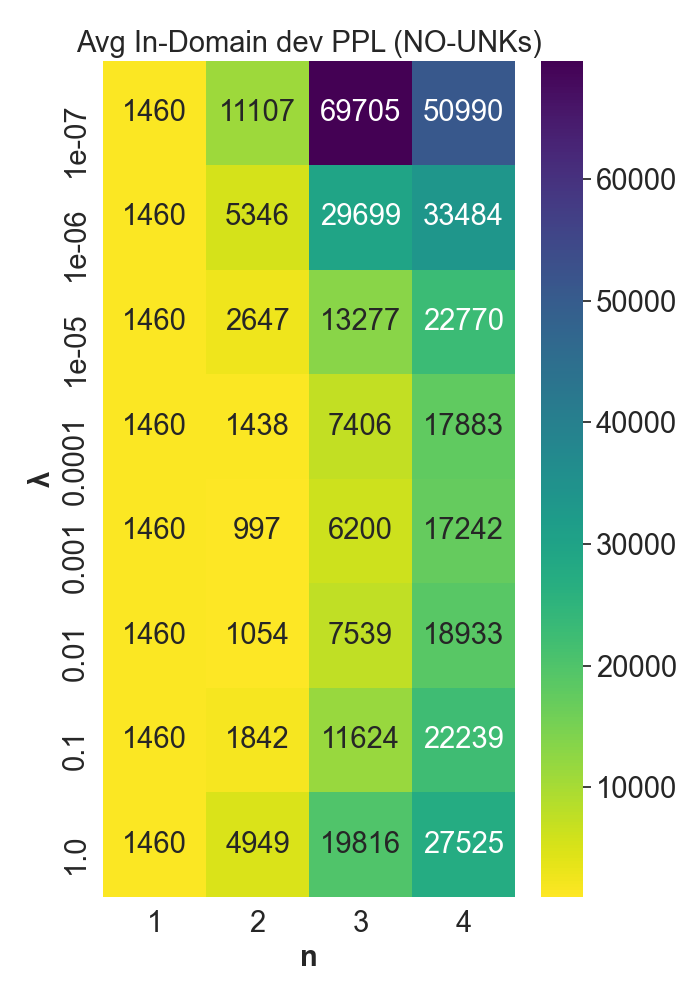
\includegraphics[width=.4\textwidth]{figures/nounks.png}
  \caption{Average In-Domain dev Perplexity for the ``no-UNKs'' model with values of $n\in\{2,3,4\}$, for varying values of $\lambda$. Performance was better than the unigram model ($n=1$)  for $n=2$ and $\lambda \in \{0.001,0.01\}$.}
  \label{fig:nounks}
\end{figure}


\begin{figure*}[ht]
\begin{subfigure}{0.5\textwidth}
  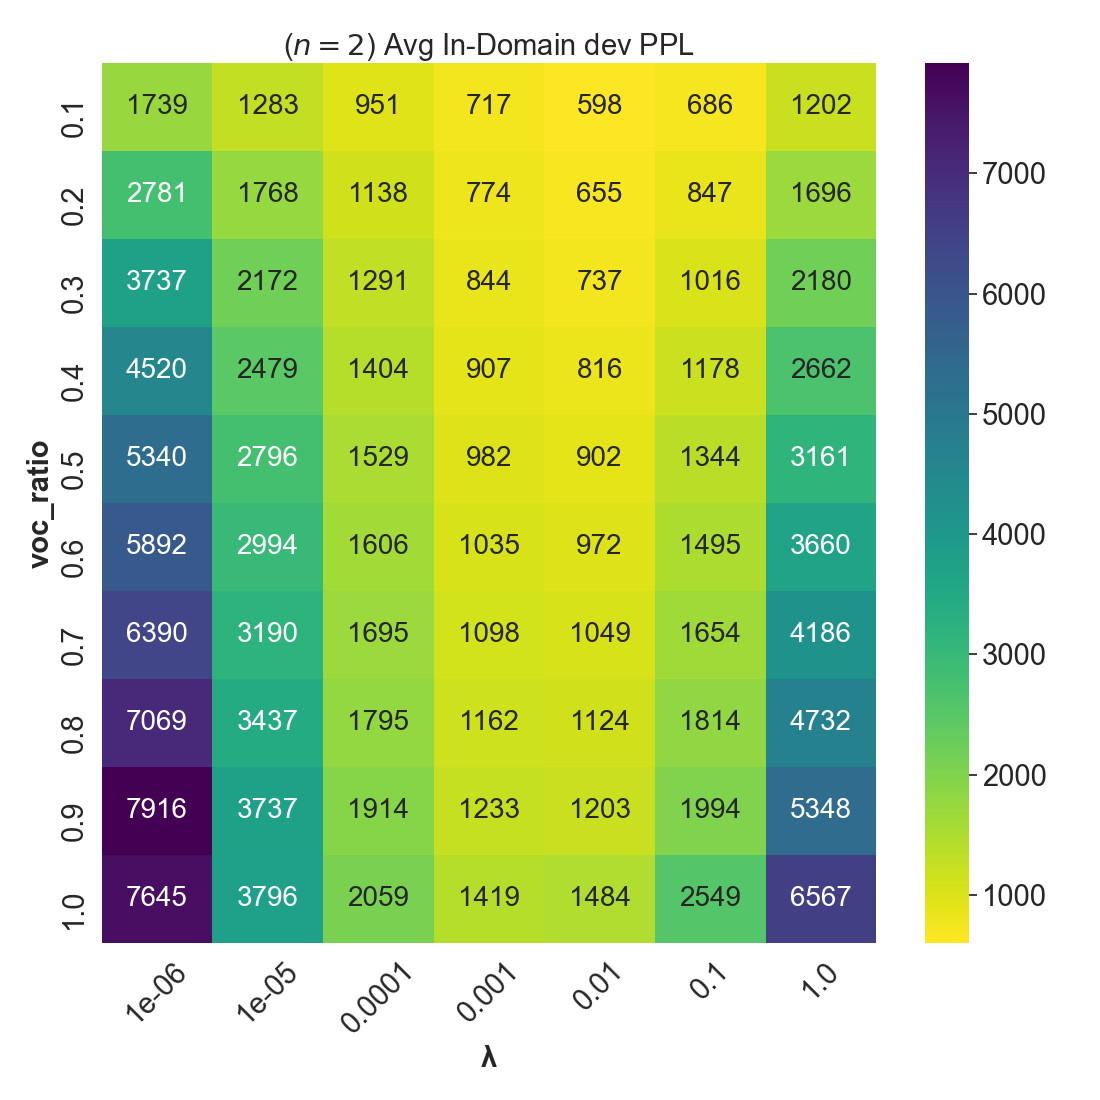
\includegraphics[width=\textwidth]{figures/n=2.png}
\end{subfigure}
\begin{subfigure}{0.5\textwidth}
  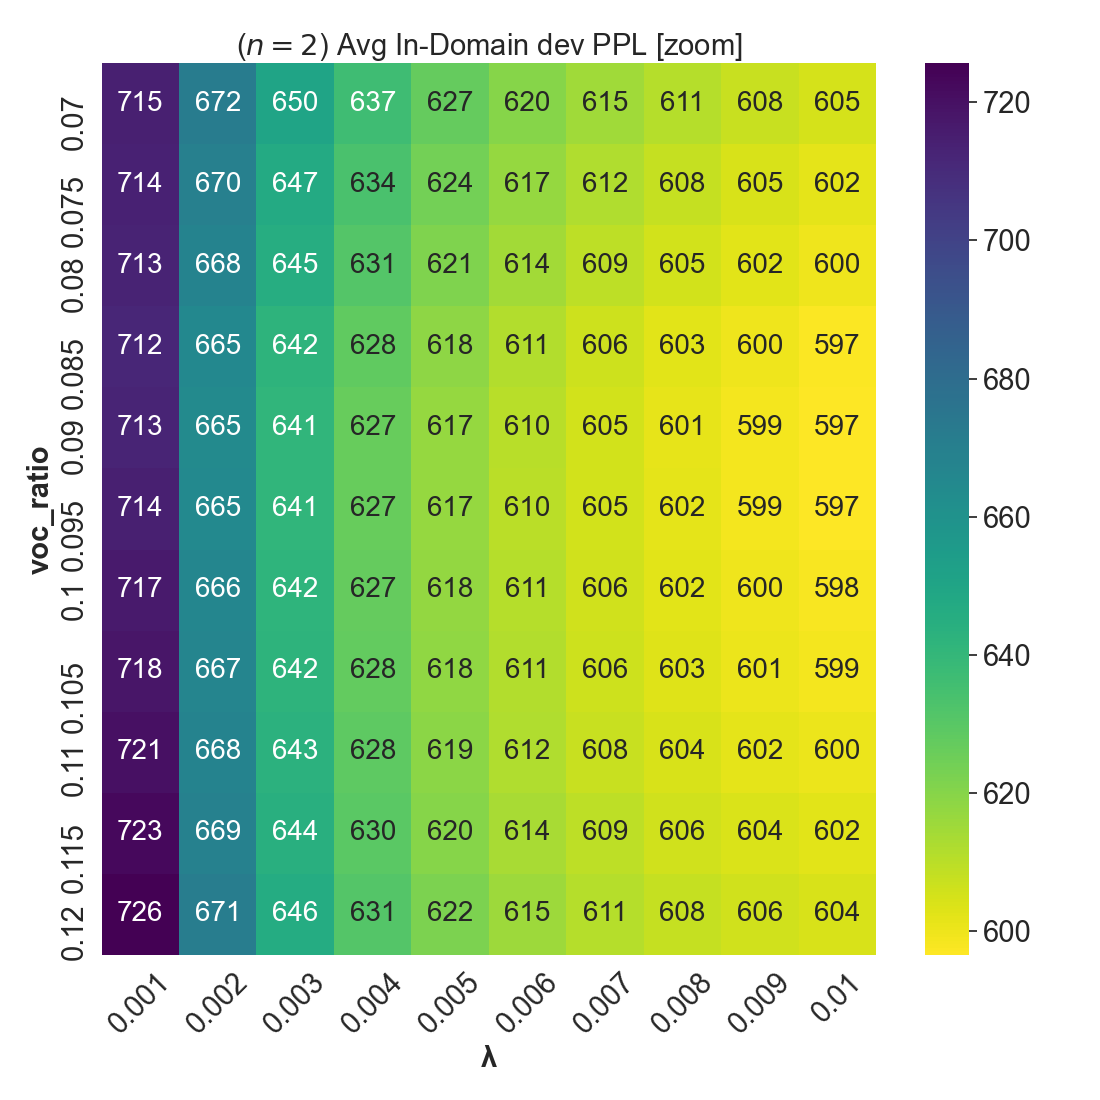
\includegraphics[width=\textwidth]{figures/n=2_zoom.png}
\end{subfigure}

\begin{subfigure}{0.5\textwidth}
  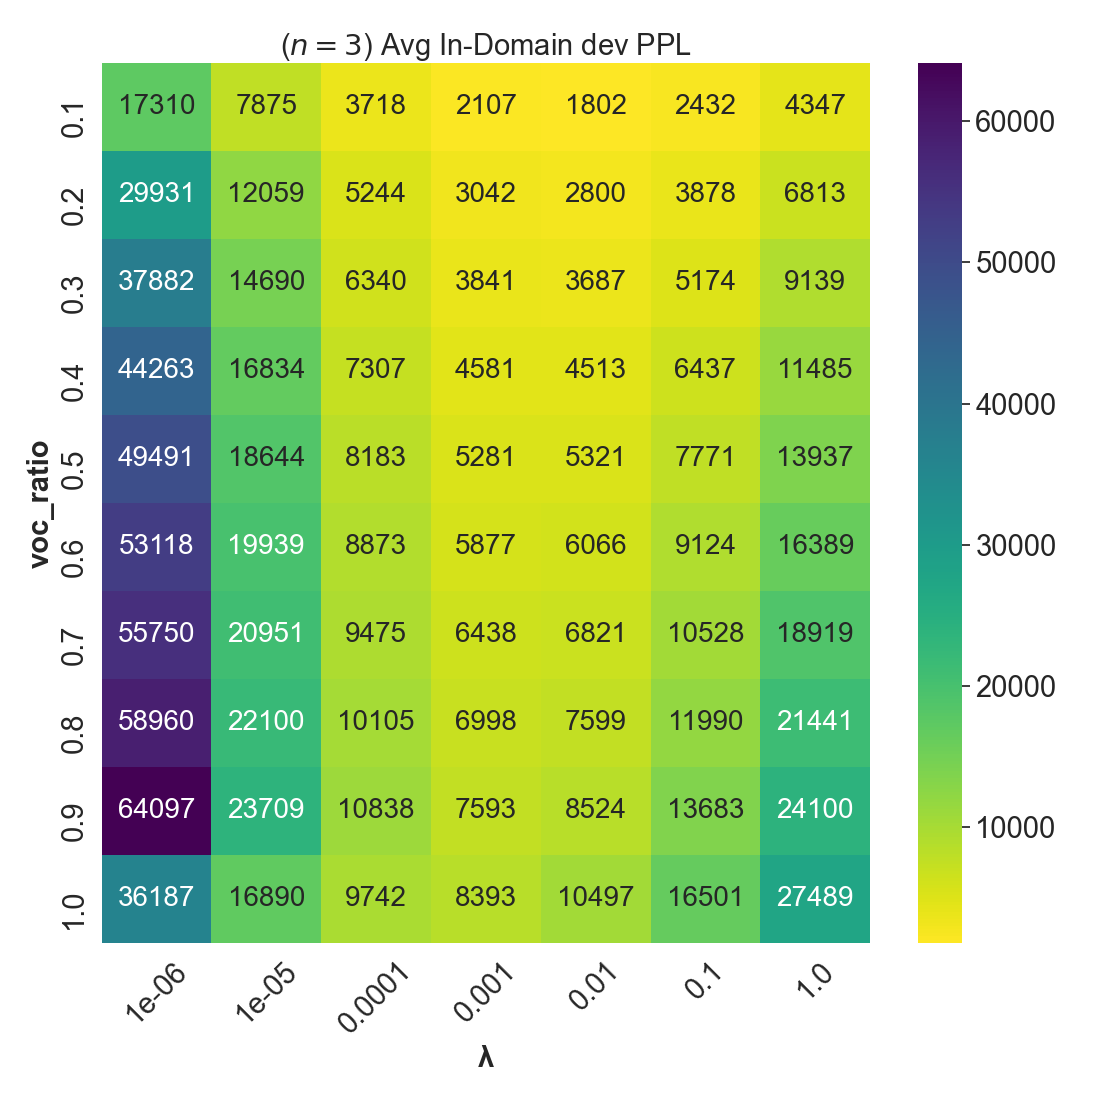
\includegraphics[width=\textwidth]{figures/n=3.png}
\end{subfigure}
\begin{subfigure}{0.5\textwidth}
  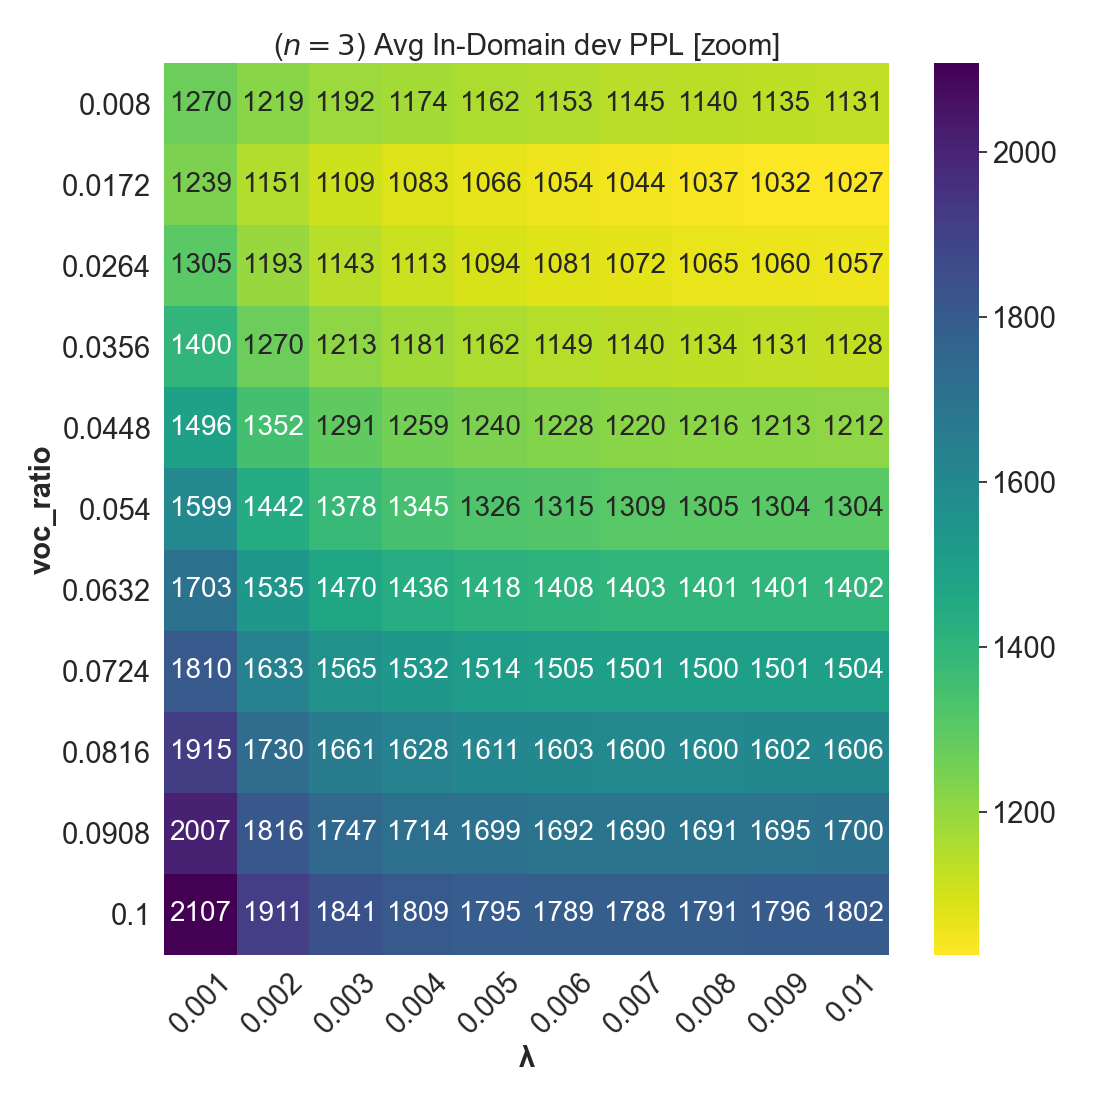
\includegraphics[width=\textwidth]{figures/n=3_zoom.png}
\end{subfigure}

\begin{subfigure}{0.5\textwidth}
  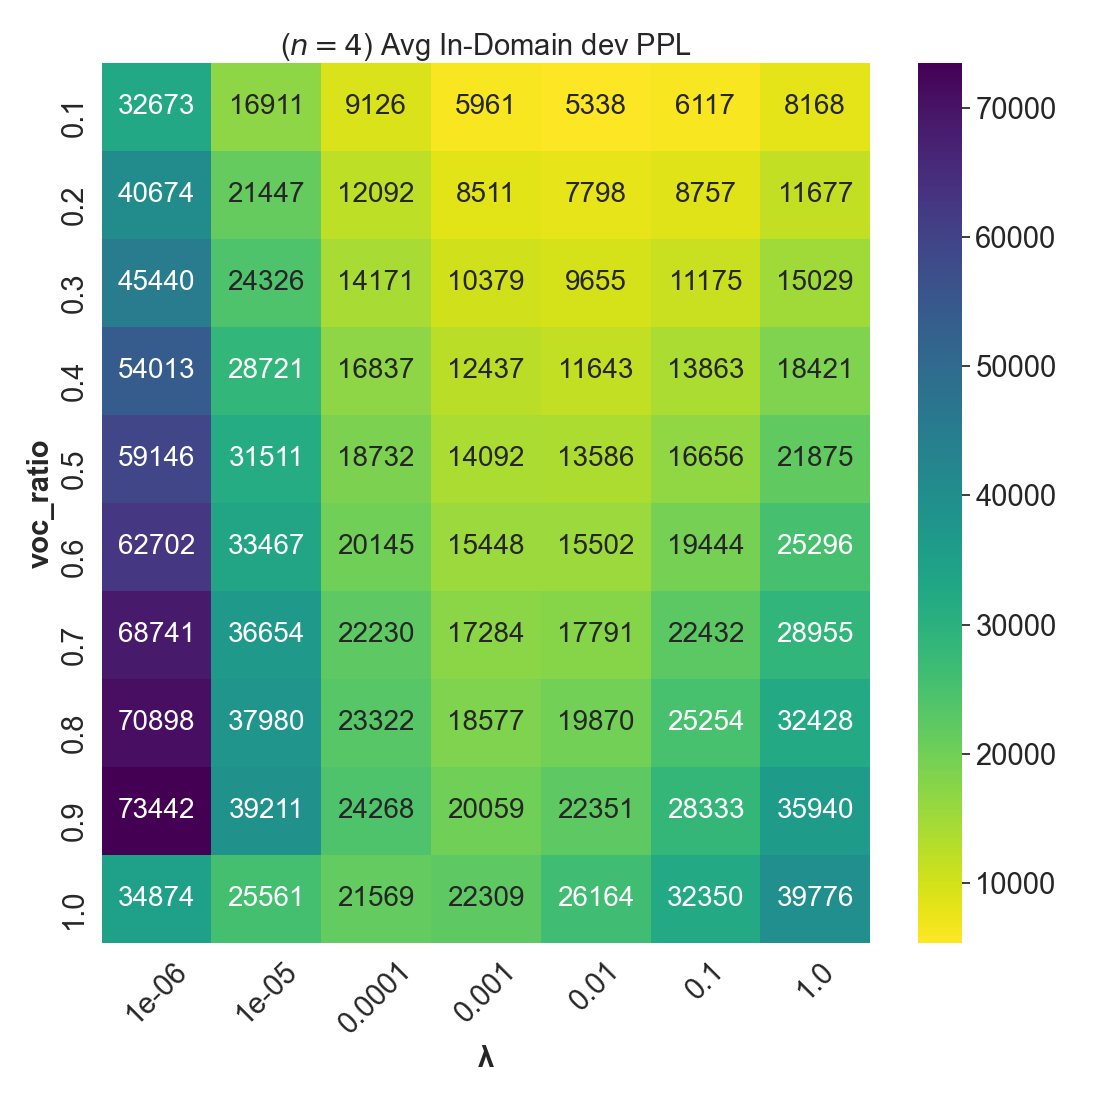
\includegraphics[width=\textwidth]{figures/n=4.png}
\end{subfigure}
\begin{subfigure}{0.5\textwidth}
  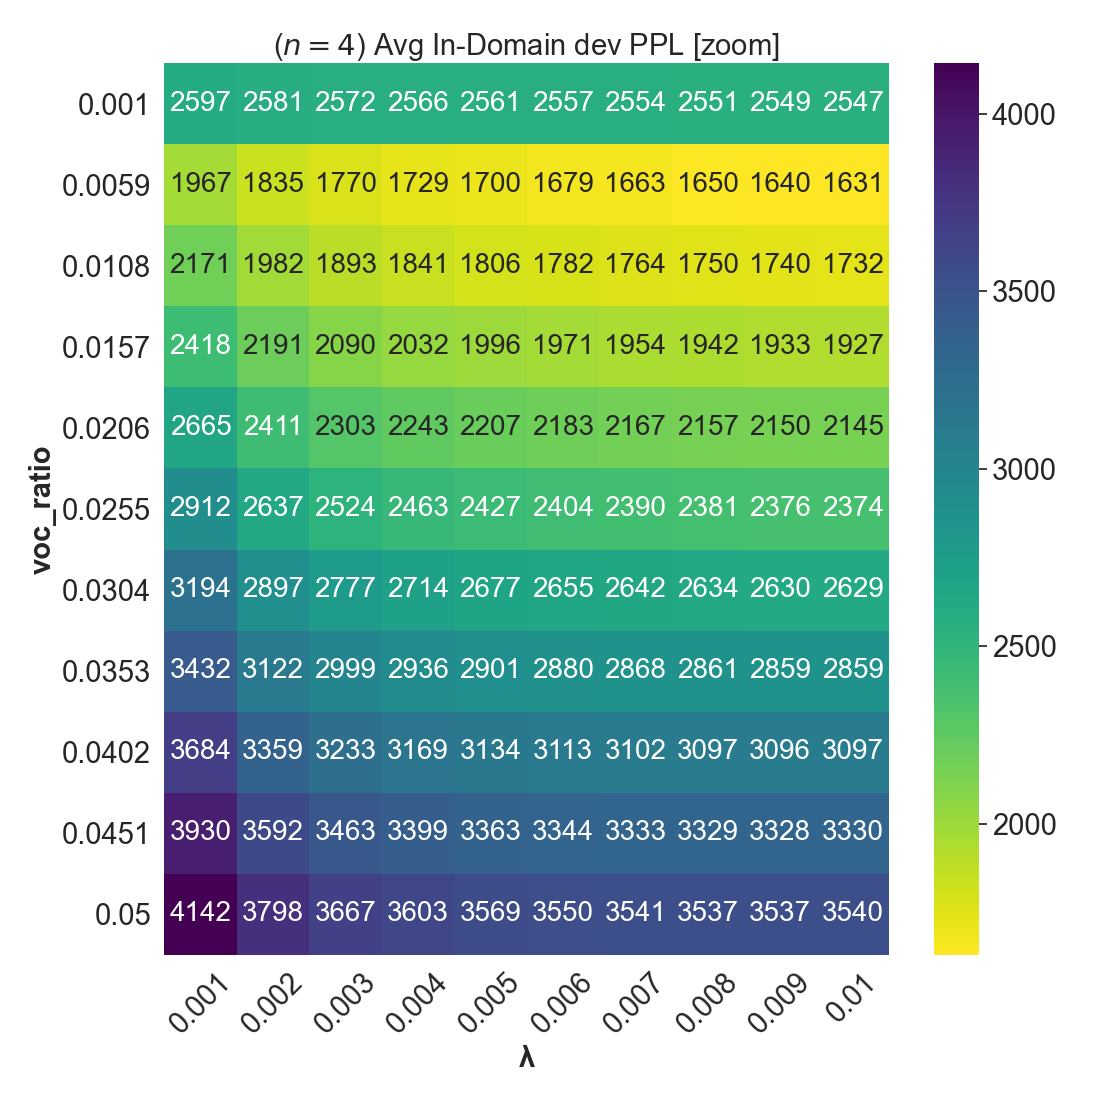
\includegraphics[width=\textwidth]{figures/n=4_zoom.png}
\end{subfigure}
\caption{Hyper-parameter search for $n$-gram models. The left column portraits initial search ranges for \textsf{voc\_ratio} and $\lambda$, and the right column portraits more fine-tuned ranges specific for each $n$, which changes across rows.}
\label{fig:search}
\end{figure*}

\FloatBarrier

\begin{figure*}
\centering
\begin{subfigure}{0.45\textwidth}
  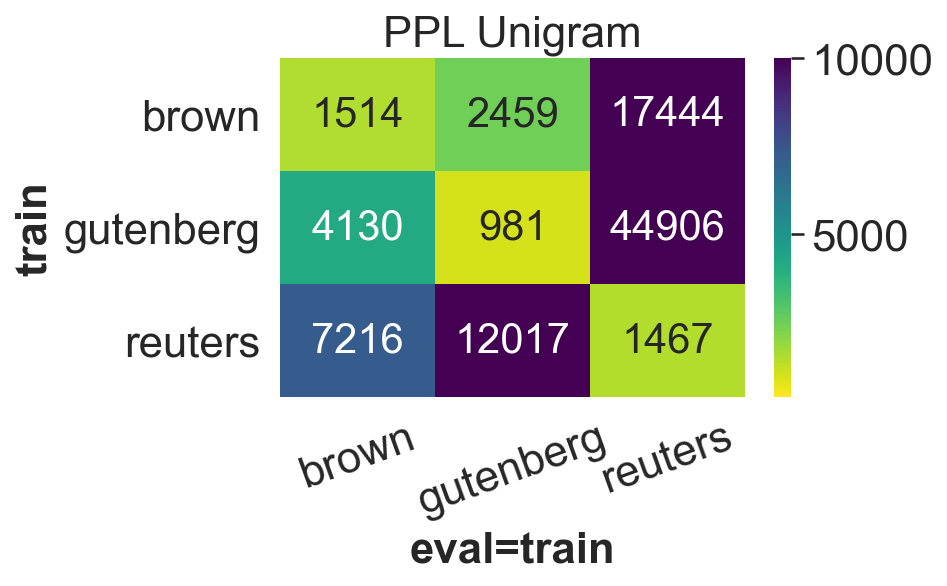
\includegraphics[width=\textwidth]{figures/unigram_cross_ppl_train.png}
\end{subfigure}
\hspace{5pt}
\begin{subfigure}{0.45\textwidth}
  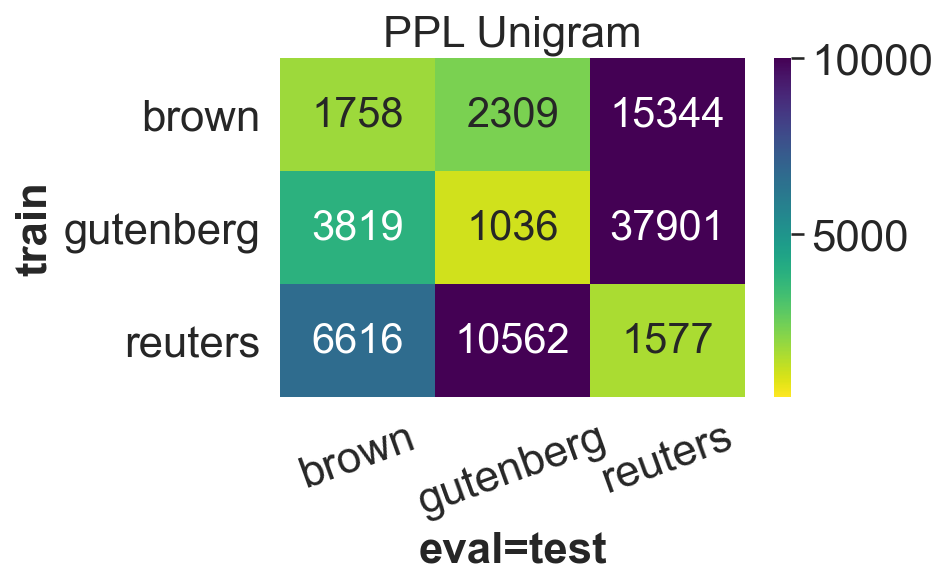
\includegraphics[width=\textwidth]{figures/unigram_cross_ppl_test.png}
\end{subfigure}

\vspace{1em}

\begin{subfigure}{0.45\textwidth}
  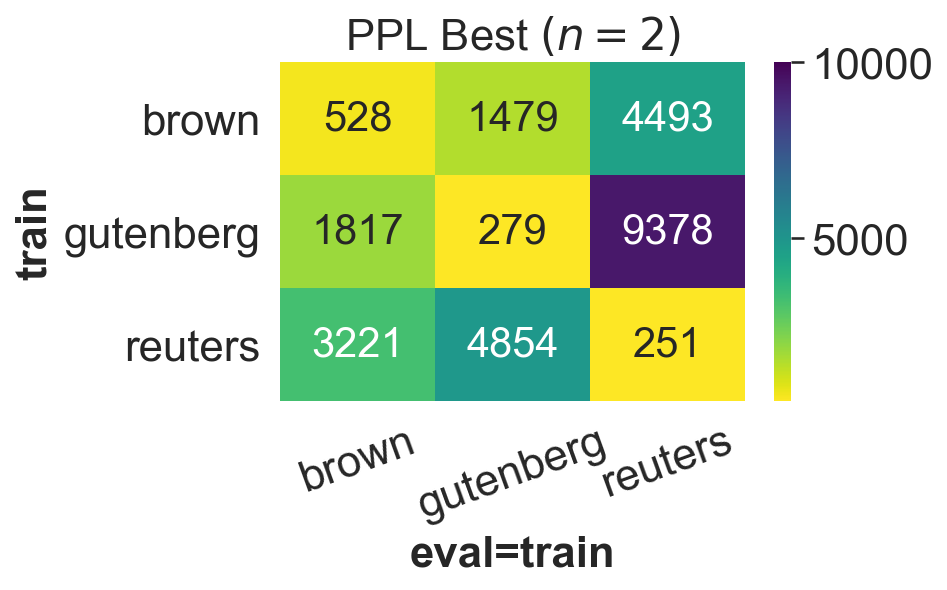
\includegraphics[width=\textwidth]{figures/bigram_cross_ppl_train.png}
\end{subfigure}
\hspace{5pt}
\begin{subfigure}{0.45\textwidth}
  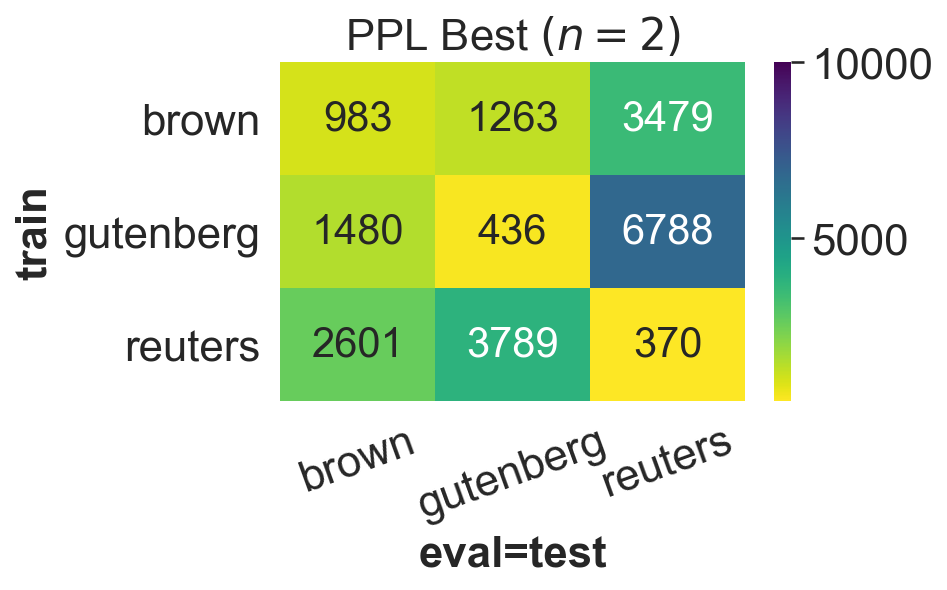
\includegraphics[width=\textwidth]{figures/bigram_cross_ppl_test.png}
\end{subfigure}
\caption{In/Cross-Domain Perplexity using train dataset (left) and test dataset (right), for the unigram model (top) and our best model $[n=2,\lambda=0.01,\textsf{voc\_ratio}=0.09]$ (bottom). Rows (resp. columns) for each case represent the dataset in which the model was trained (resp. evaluated).}
\label{fig:cross_ppl}
\end{figure*}


\begin{table*}
\centering
%!TEX root=report.tex
\begin{tabular}{c||c|r|l||c|r|l}
  \multirow{2}{*}{\textbf{Domain}} & \multicolumn{3}{c||}{\textbf{unigram > bigram}} & \multicolumn{3}{c}{\textbf{unigram < bigram}} \\\cline{2-7}
  & \textbf{Model} & \textbf{PPL} & \textbf{Sentence} & \textbf{Model} & \textbf{PPL} & \textbf{Sentence}\\\hhline{=||=|=|=||=|=|=}
  %
  \multirow{2}{*}{Brown} & unigram & 287 & \multirow{2}{*}{That one they would} & unigram & 2727 & \multirow{2}{*}{The quick brown fox jumps.} \\
                         & bigram  & 1371 &                                     & bigram  & 439 & \\\hline
  %
  \multirow{2}{*}{Gutenberg} & unigram & 412 & \multirow{2}{*}{Israel 15 and 16 from him.} & unigram & 372 & \multirow{2}{*}{The people of Israel did it.} \\
                         & bigram  & 10781 &                                     & bigram  & 54 & \\\hline
  %
  \multirow{2}{*}{Reuters} & unigram & 429 & \multirow{2}{*}{It has shares of him of 000.} & unigram & 1616 & \multirow{2}{*}{His financial analyst is rich.} \\
                         & bigram  & 1421 &                                     & bigram  & 222 & \\
\end{tabular}

\caption{Comparison of sentences generated across domains to highlight differences/similarities between the unigram and our best bigram model.}\label{tbl:uniVsBi}
\end{table*}

\begin{table*}
\centering
%!TEX root=report.tex
\begin{tabular}{c|r|l||c|r|l}
  \multicolumn{3}{c||}{\textbf{Brown > Reuters}} & \multicolumn{3}{c}{\textbf{Brown < Reuters}} \\\hline
  \textbf{Domain} & \textbf{PPL} & \textbf{Sentence} & \textbf{Model} & \textbf{PPL} & \textbf{Sentence}\\\hhline{=|=|=||=|=|=}
  %
  Brown     & 260 & \multirow{2}{*}{This love for God.} & Brown      & 405 & \multirow{2}{*}{The company code is 000.} \\
  Reuters   & 3278 &                                    & Reuters    & 41 & \\\hhline{=|=|=||=|=|=}
  %
  \multicolumn{3}{c||}{\textbf{Brown > Gutenberg}} & \multicolumn{3}{c}{\textbf{Brown < Gutenberg}} \\\hline
  Brown     & 45 & \multirow{2}{*}{American of the year.} & Brown      & 898 & \multirow{2}{*}{God though shall not.} \\
  Gutenberg & 141 &                    & Gutenberg  & 237 & \\\hline
\end{tabular}

\caption{Comparison of sentences generated by our best bigram model to highlight differences/similarities between domains.}
\label{tbl:compDomains}
\end{table*}

\FloatBarrier


\begin{table*}
\vspace{-50pt}
%!TEX root=report.tex
\begin{tabular}{c|c|l}
  \textbf{Domain} & \textbf{Model} & \textbf{Sentence} \\\hline
  \multirow{2}{*}{Brown} & bigram & remarked heads Mantle pair of her father and larger filled eyes \\
  & unigram & home doorway friendly In of the after good goal pictures the \\ \hline
  \multirow{2}{*}{Gutenberg} & bigram & with you look which also of jewels blind whoever walks silently \\\
  & unigram & olive it out Street the God awhile and if get Weston \\\hline
  \multirow{2}{*}{Reuters} & bigram & the central going to follow not cover losses running at 125 \\
  & unigram & lt see year mln providing face appointed payment and reached ahead \\\hhline{|=|=|=|}
  \multirow{2}{*}{Brown}  & bigram & \emph{The} engineering contributions of my own when the Greek  practical \\
   & unigram & \emph{The} fit League stands the Hillsboro to to apogee \\\hline
  \multirow{2}{*}{Gutenberg} & bigram & \emph{The} wise man that saw yet \\\
   & unigram & \emph{The} the to is king and to as Father laid Chinese \\\hline
  \multirow{2}{*}{Reuters} & bigram & \emph{The} company with Saudi Arabia was 19 billion francs vs 50 \\
   & unigram & \emph{The} Strata to shares ON governments marks bank as that that \\\hhline{|=|=|=|}
  \multirow{2}{*}{Brown}  & bigram & \emph{I} and exciting new house and that the dollar being  \\
   & unigram & \emph{I} the England \\\hline
  \multirow{2}{*}{Gutenberg} & bigram & \emph{I} in God walk at the ground they shall not absolutely \\\
   & unigram & \emph{I} where play and time But he which my ashamed Captain \\\hline
  \multirow{2}{*}{Reuters} & bigram & \emph{I} is wholly associated with investors and earnings for the reserves \\
   & unigram & \emph{I} in Outokumpu 000 Marathon of \\\hhline{|=|=|=|} 
  \multirow{2}{*}{Brown} & bigram & \emph{How} grateful to its members at all our eyes but for \\
   & unigram & \emph{How} with when grooved Andy party we bad Leonato of experimental \\\hline
  \multirow{2}{*}{Gutenberg} & bigram & \emph{How} does that which think might end it ceased \\\
   & unigram & \emph{How} the because \\\hline
  \multirow{2}{*}{Reuters} & bigram & \emph{How} IN 1987 projected money market agreed to cost speaking for \\
   & unigram & \emph{How} The this But Inc little said January to the pieces \\\hhline{|=|=|=|} 
  \multirow{2}{*}{Brown}  & bigram & \emph{Financial} of members to be there \\
   & unigram & \emph{Financial} incident than the Mantle similar of on problem these \\\hline
  \multirow{2}{*}{Gutenberg} & bigram & \emph{Financial} How dare passeth among those which is ready for us \\\
   & unigram & \emph{Financial} to 27 saying and house by negro not really walking \\\hline
  \multirow{2}{*}{Reuters} & bigram & \emph{Financial} Corporation targets such holding company said \\
   & unigram & \emph{Financial} 20 DLRS holding The the dollar policy \\\hhline{|=|=|=|} 
  \multirow{2}{*}{Brown}  & bigram & \emph{God} existing About three 26 editorial and the two kids  \\
   & unigram & \emph{God} examined \\\hline
  \multirow{2}{*}{Gutenberg} & bigram & \emph{God} created papa \\\
   & unigram & \emph{God} hide happened and encourager of and shake that he fairly \\\hline
  \multirow{2}{*}{Reuters} & bigram & \emph{God} recent offers Morgan applications trend is for 12 14 days \\
   & unigram & \emph{God} the and 50 to the \\\hhline{|=|=|=|} 
  \multirow{2}{*}{Brown}  & bigram & \emph{God is} something that thou shalt not imagine you wives  \\
   & unigram & \emph{God is} night 16 the therewith busy which the father not \\\hline
  \multirow{2}{*}{Gutenberg} & bigram & \emph{God is} itself \\\
   & unigram & \emph{God is} education the Psychologically shall in \\\hline
  \multirow{2}{*}{Reuters} & bigram & \emph{God is} more competitive production last year or be temporary reserves \\
   & unigram & \emph{God is} income suit season to JAN nations \\\hhline{|=|=|=|} 
  \multirow{2}{*}{Brown}  & bigram & \emph{The man} has shown steady purpose of society \\
   & unigram & \emph{The man} satisfactorily an of six months although with columns without \\\hline
  \multirow{2}{*}{Gutenberg} & bigram & \emph{The man} who should do work sake For the servants were \\\
   & unigram & \emph{The man} Will 11 vex neuer do always \\\hline
  \multirow{2}{*}{Reuters} & bigram & \emph{The man} in the previous business involved but the Securities and \\
   & unigram & \emph{The man} sales 1985 it increase Only Salvino declining the GCC \\\hhline{|=|=|=|} 
  \multirow{2}{*}{Brown}  & bigram & \emph{I love} him in shore gun symbol of the Church \\
   & unigram & \emph{I love} these was even an of demanded children to Low \\\hline
  \multirow{2}{*}{Gutenberg} & bigram & \emph{I love} you in moment afterwards by man died in Pharaoh \\\
   & unigram & \emph{I love} is were Have He was scheme previous this creep \\\hline
  \multirow{2}{*}{Reuters} & bigram & \emph{I love} financial rand from August Six mths Shr six cts \\
   & unigram & \emph{I love} five at Senate able to Metex For bid international
\end{tabular}

\caption{Sentences generated by both the unigram and our best bigram model. Prefixes given to each simulation are highlighted, except for the first case where the prefix was empty.}\label{tbl:generated}
\end{table*}




\end{document}
